 \documentclass[oneside,letter,11pt]{article}

%% The graphicx package provides the include graphics command.
\usepackage{graphicx}
%% The amssymb package provides various useful mathematical symbols
\usepackage{amssymb}
%% The amsthm package provides extended theorem environments
%% \usepackage{amsthm}

%% The lineno packages adds line numbers. Start line numbering with
%% \begin{linenumbers}, end it with \end{linenumbers}. Or switch it on
%% for the whole article with \linenumbers after \end{frontmatter}.
\usepackage{enumitem}

\newlist{deflist}{description}{2}
\setlist[deflist]{labelwidth=2cm,leftmargin=!,font=\normalfont}
\usepackage{comment}
\usepackage{enumerate}
\usepackage{lineno}
\usepackage{tikz}
\usetikzlibrary{matrix}
\usetikzlibrary{positioning}
\usepackage{xcolor}
\usepackage{amsmath}
\usepackage{mathtools}
\usepackage{blkarray, bigstrut}
\usepackage[T1]{fontenc}
\usepackage[utf8]{inputenc}
\usepackage{mathtools}
\usepackage{blkarray, bigstrut}
\usepackage{gauss}
\usetikzlibrary{arrows.meta}
\usetikzlibrary{shapes,backgrounds}
\usetikzlibrary{decorations.text}
\usetikzlibrary{decorations.text,calc,arrows.meta}
\usepackage{multirow}
\usepackage{float}
\usepackage{svg}
\usepackage{graphicx}
\usepackage{subfig}
\usepackage{epstopdf}
\usepackage{soul}

\linespread{1.2}

\usepackage[top=1 in, bottom=1 in, left=1 in, right=1 in]{geometry}


\newtheorem{theorem}{Theorem}
\newtheorem{lemma}{Lemma}
\newtheorem{proposition}{Proposition}
\newtheorem{corollary}{Corollary}
\newtheorem{definition}{Definition}
\newtheorem{example}{Example}


% Paragraphs: Indent first line 12.7 mm (0.5 in.); do not use an extra line space between paragraphs; do not indent first line after a subhead
\setlength{\parindent}{0.5in}

% Subheads: All subheads should be flush with the left margin, with one line space above
\usepackage[tiny]{titlesec}
% FIRST-LEVEL SUBHEAD (all capitals, boldface, on separate line)
\titleformat{\section}{\bf}{}{0pt}{\uppercase}
\titlespacing*{\section}{0pt}{\baselineskip}{0pt}
% Second-Level Subhead (initial capitals, boldface, on separate line)
\titleformat{\subsection}{\bf}{}{0pt}{}
\titlespacing*{\subsection}{0pt}{\baselineskip}{0pt}
% Third-Level Subhead (initial capitals, italic, on separate line)
\titleformat{\subsubsection}{\it}{}{0pt}{}
\titlespacing*{\subsubsection}{0pt}{\baselineskip}{0pt}
% Fourth-Level Subhead (initial capitals, boldface, on same line as text, with extra letter space between the subhead and text)
\titleformat{\paragraph}[runin]{\bf}{}{}{}[]
\titlespacing*{\paragraph}{0pt}{\baselineskip}{1em}
% Fifth-Level Subhead (initial capitals, italic, on same line as text, with extra letter space between the subhead and text)
\titleformat{\subparagraph}[runin]{\it}{}{}{}[]
\titlespacing*{\subparagraph}{0pt}{\baselineskip}{1em}

% Bulleted and numbered lists: Indent first line 12.7 mm (0.5 in.); do not indent text runovers.
%% Translation by FvW: lists should look just like paragraphs:
\usepackage{paralist}
\renewcommand{\itemize}{\asparaitem}
\renewcommand{\enumerate}{\asparaenum}
\renewcommand{\description}{\asparadesc}


\usepackage{ccaption}
\makeatletter
\renewcommand{\fnum@table}[1]{\textbf{TABLE~\thetable} \hspace{1em} }
\renewcommand{\fnum@figure}[1]{\textbf{FIGURE~\thefigure} \hspace{1em} }
\makeatother
\captiontitlefont{\bfseries}

% Line numbering (not prescibed but kindly asked for to make review easier)

\usepackage{times}

\usepackage[pagewise]{lineno}
\modulolinenumbers[2]
\linenumbers


\pagestyle{myheadings}
\markright{\small Shanto and Li \hfill}

% \usepackage{booktabs} % FvW: makes tables look nicer

%\usepackage{subfigure} % FvW: to make subfigures

\usepackage{tikz} % FvW: to make very nice looking graphs

% \usepackage[colorlinks,breaklinks]{hyperref} % FvW: makes clickable references/citations/urls 
% \urlstyle{same}

\usepackage{amsmath} 
\usepackage[capposition=top]{floatrow}

\begin{document}

\rm



\title{Mixed Traffic Flow of Human-Driven and Autonomous Vehicles: Self-organized Clustering and Lane Formation}


\author{
\\
\\
\\
\\
\\
Sadman Ahmed Shanto\\
Department of Physics and Astronomy\\
Texas Tech University\\
Phone: 806-790-0156\\
Email: sadman-ahmed.shanto@ttu.edu \\
\vspace{3ex}\\
Jia Li, Ph.D.\\
(Corresponding Author)\\
Department of Civil, Environmental, and Construction Engineering\\
Texas Tech University\\
Phone: 806-834-8291\\
Email: jia.li@ttu.edu\\
\vspace{3ex}
}
\date{
Paper submitted to TRB Annual Meeting 2020 \\
\medskip \\
August 1, 2019\\
\medskip\\
4500 words + 14 figure(s)$\times$ 0 + 3 table(s) $\times$ 250 $=$ 5250 words \\
}


\thispagestyle{empty}
\maketitle
\newpage


%%
%% ABSTRACT, max 250 words
%%

\section*{Abstract}

\textcolor{red}{Add any numbers if possible and talk about opportunistic behavior leading to clustering\\}
This paper reveals the existence of self-organized clustering (platooning) and lane formation in mixed traffic flow of autonomous vehicles (AVs) and human-driven vehicles (HVs) based on simulation experiments. We propose a parsimonious Cellular Automata model to capture the different characters of AVs and HVs as well as their interactions. AVs are endowed with opportunistic behaviors, reflected through gap seeking and awareness of neighbor vehicle types. We compare clustering and lane formation properties and mixed flow flux in three scenarios, accounting for the impact of two distinct AV behavior types and a control case of homogeneous flow. We observe that, intriguingly, even with this relatively simple model, AVs demonstrate self-organized properties in the mixed traffic flow. AVs form into clusters (i.e. platoons) and even lanes on their own in the mixed flow, without centralized control. Such phenomena seem to relate to the intrinsic incentives that AVs perceive and their ability to tell neighbor vehicle types. This finding suggests the possibility of regulating mixed AV-HV flow through distributed incentives, rather than centralized coordination.


\newpage

%%
%% MAIN TEXT
%%

\thispagestyle{empty}

\section{Introduction}\label{S:1}

% \textcolor{blue}{[expand the abstract, present literature, and highlight contributions]}

% general background
Driver-less cars (i.e. autonomous vehicles, henceforth called AVs) have already appeared on the road and shared right of way with human-driven vehicles (henceforth called HVs). An appealing feature of AVs is their capability to form platoons, which is anticipated to boost efficiency of traffic flow substantially. A number of recent research have delved into modeling and operations of the mixed flow of AVs and HVs, most of them attempted to capture or optimize the platooning feature of AVs. 

Much attention in literature (see e.g. \cite{bose2003analysis}\cite{talebpour2016influence}\cite{olia2018traffic}\cite{wang2014rolling}\cite{gong2016constrained}\cite{zhou2017parsimonious}) has focused on problems along the longitudinal dimension and adopt a microscopic approach, which embraces simulation of car-following behaviors, platoon control, and stability analysis. While the understanding of microscopic longitudinal behaviors of mixed AV-HV flow has become relatively mature, the collective behaviors to be anticipated in a multi-lane setting remain elusive, where the interplay of AVs and HVs can be substantially more complicated, due to the possibility of lane choice and lane changing. The lateral behaviors are coupled with longitudinal dynamics, and the two together determine dynamics of mixed AV-HV flow. Discussions along this line are still primitive, mostly focused on the estimation of mixed flow capacity (see e.g. \cite{chen2017towards}\cite{ghiasi2017mixed}) and aggregate flow-density relation (see e.g. \cite{rao1993flow}\cite{levin2016multiclass}). These works all assume the mixed flow is in perfect steady state does not explicitly consider lateral interactions in general multilane setting. Concerning the impacts of lanes on traffic flow, several empirical studies \cite{menendez2007effects}\cite{daganzo2008effects}\cite{cassidy2009spatiotemporal}\cite{cassidy2010smoothing} have been conducted towards understanding the impacts of HOV lanes on traffic in general purpose (GP) lanes, which revealed the existence of a smoothing effect caused by restriction of lane-changing. Past research also examines lane-to-lane traffic interactions on multilane highways, which include lane flow distribution \cite{michalopoulos1984multilane}\cite{shiomi2015multilane}, as well as impacts of microscopic lane-changes \cite{laval2006lc}\cite{ahn2007freeway}. On the theoretical side, it is only in limited cases that the connection between lane policy and traffic flow characteristics has been investigated, and in almost all studies, the policy considered is static. \cite{daganzo1997continuum} and \cite{jin2018new} both considered traffic consisting of regular and priority vehicles, and a number of special lanes are accessible only to the priority vehicles. Both regular vehicles and priority vehicles are endowed with the identical fundamental diagram. Nonetheless, these studies are focused on human-driven traffic flow and do not consider any AV-specific behaviors. \cite{chen2017towards} discussed capacity of mixed flow of AVs and HVs on multi-lane freeway under different combination of static lane access policies, assuming traffic flow is steady. \cite{ghiasi2017mixed} derived capacity of mixed AV-HV flow in a similar context, assuming the spatial distribution of mixed flow follows a Markov process. An interesting lateral policy considered in literature is intermittent bus lane (IBL), which offers priority to buses, but also allows other regular vehicles to use the lane when space is available. \cite{eichler2006bus} and \cite{chiabaut2012road} conducted queuing analysis using the LWR model and derived corresponding roadway capacity as well as conditions when IBL will benefit the entire system.

The key challenge to model mixed flow dynamics of AVs and HVs lies in capturing agents' longitudinal and lateral behaviors simultaneously, which should account for not only agents' dynamical characters (e.g. their longitudinal speed and acceleration as functions of headway), but also agents' decision-making, as well as  how the decisions of individual agents aggregate. Such interactions in mixed flow of AVs and HVs is conceivably more complicated than mixed human-driving traffic due to the rich possibilities of AV behaviors. For instance, with the advanced sensing and communication capabilities, AVs may behave more opportunistically than HVs in seeking peers in its neighborhood, because this potentially allow them to form platoons with peers and benefit from more smooth driving and better traveling speed. 


In this paper, we are interested in understanding the collective dynamics of AV-HV flow, as a result of the interactions between heterogeneous agents. In particular, we seek to answer the following research questions: when AVs are self-interested and individually controlled by themselves (as opposed to coordinated by system operator), will they be able to self-organize into platoons? And if so, what are the conditions for the self-organization to initiate and sustain? This research is partly inspired from the self-organized phenomena widely existing in biological systems, such as army ants \cite{couzin2003self}, where orders emerge when agents interact with each other locally. In traffic flow literature, similar self-organized phenomena were also reported \cite{helbing2001traffic}.


To answer the above questions, we propose a Cellular Automaton (CA) model to encapsulate the essential behavioral factors of AVs and HVs, and conduct simulation experiments to characterize the impact of these behavior factors on the formation of clusters in mixed traffic flow. The simulation experiments were conducted on a circular road with three lanes. We consider two alternatives of AV behaviors. In the first scenario, AVs behave like HVs, except the difference in free flow speed and braking probability. In the second scenario, AVs are assumed to be fully aware of vehicle types in neighborhood and opportunistic in gap seeking.


The major finding of this research is the self-organized formation of AV clusters and lanes without any centralized control. This finding may suggest clustering as an intrinsic property of mixed flow, when AVs and HVs interact, and AVs are endowed with opportunistic behaviors. The existence of self-organization, if turns out to exist in real mixed flow of AVs and HVs, may suggest the possibility of regulating their interactions through a decentralized approach. 

% research gap & research contribution


% paper organization
The remaining part of the paper is organized as follows. We first introduce how we capture the different car-following and gap seeking behaviors of AVs and HVs through a Cellular Automata (CA) model. Then we describe the setup of simulation experiments along with results and discussion. In this section, we focus on the flux of mixed flow as well as the formation process of AV clusters in different behavioral scenarios. Self-organized behaviors are observed in both models of AV behavior. We summarize the findings and remark on future works in the last section.



\section{Cellular Automata Model}\label{S:2}

Cellular Automata (CA) is a simple yet effective framework to model agent interactions over cells, which have found wide and successful applications modeling traffic flow. In CA, each agent occupies a cell, and its behavior is determined by its own state and the state of other agents in its neighborhood. Simple functions can be applied to these cell objects to change its state and as a result it can change the states of neighboring cells \cite{CAb}. Nagel and Schreckenberg (1992)  were amongst the first to use this computational technique to model traffic flow \cite{CA}. 
\begin{comment}
\begin{figure}[H]
\centering
  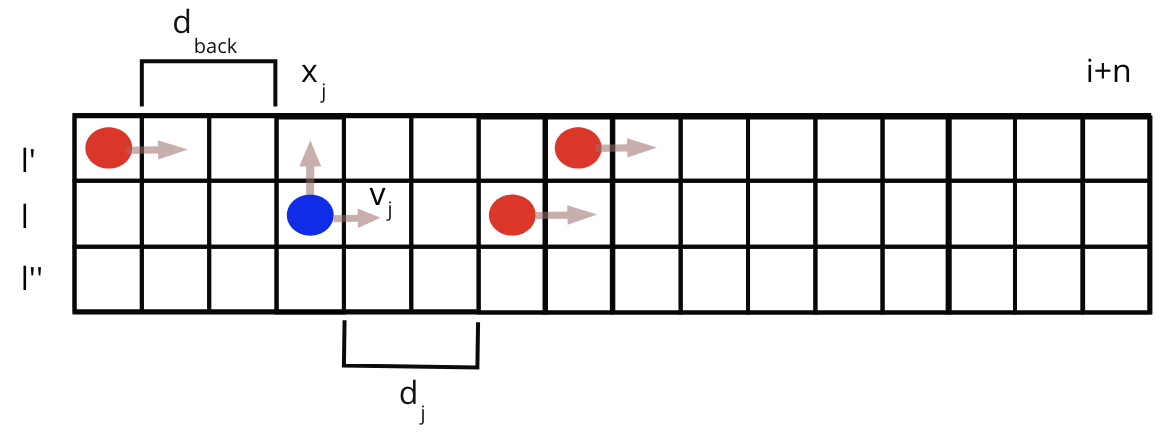
\includegraphics[width= 0.425\textwidth]{l2.png}
  \vspace{-0.3cm}
  \caption{Road - Car grid in Cellular Automata}
    \vspace{-0.2cm}
  \label{fig:lane}
\end{figure}
\end{comment}


The CA model in traffic flow literature comprises a system of vehicles that evolve over linear time in accordance to rules (see e.g. \cite{CA2}\cite{NaSch}) summarized in Fig.\ref{fig:ca}; where, $v_{j}$ represents the speed of the car $j$, $v_{max}$ is the speed limit of the road, $d_{j}$ is the number of empty cells in front of car $j$, $x_{j}$ is the cell that car $j$ occupies, $v_{l'}$ is the number of empty cells in front of car $j$ if it were on lane, $l'$, and $d_{back}$ is the number of empty cells behind in the car in lane $l'$. Each update of the system, requires all the vehicles to follow these rules simultaneously, with each vehicle first deciding whether to change lane before deciding how much to move forward; this order of decision making is fundamental to the CA model.

\begin{figure}[H]
  \centering
  \subfloat[rules for single-lane highway]{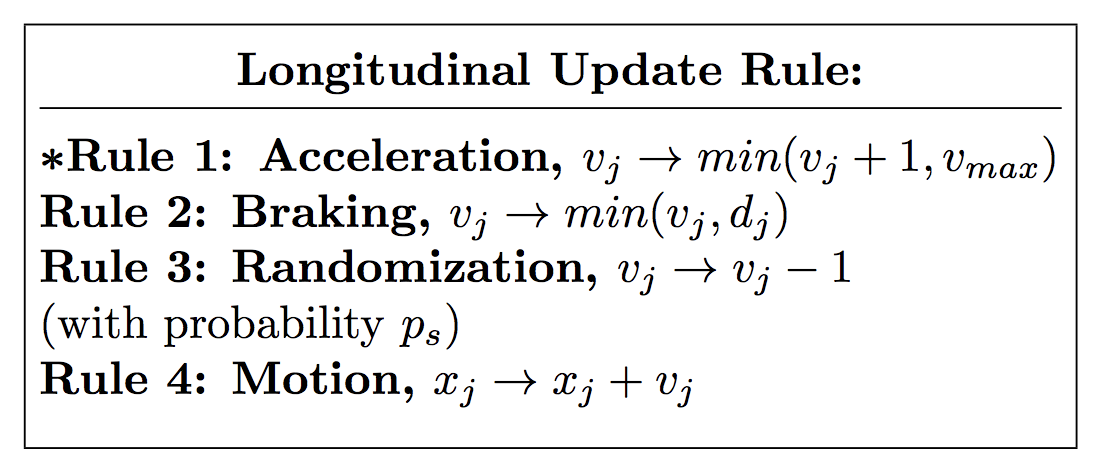
\includegraphics[width=0.5\textwidth]{v1.png}\label{fig:ca1}}
  \hfill
  \subfloat[rules for multi-lane highway]{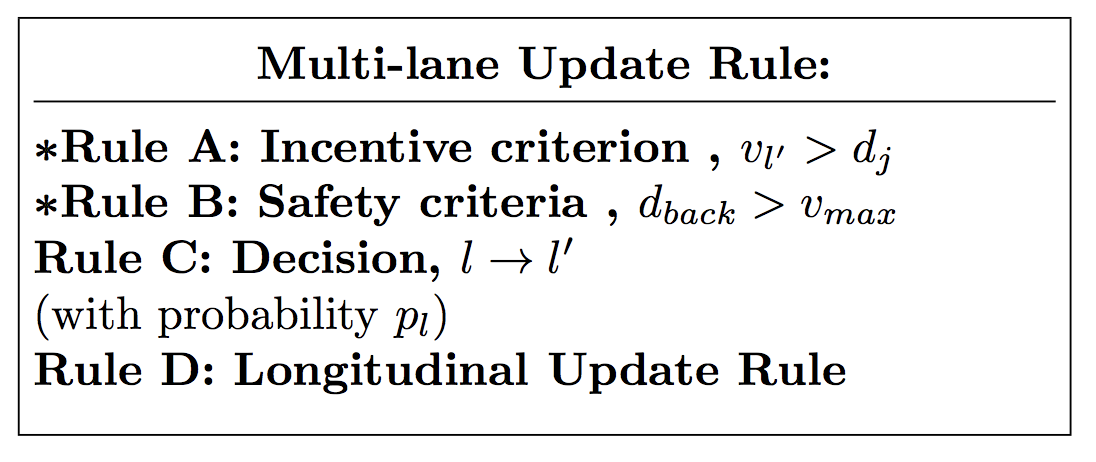
\includegraphics[width=0.5\textwidth]{v2.png}\label{fig:ca2}}
  \caption{Rules for CA models for traffic flow}
  \label{fig:ca}
\end{figure}


\\In this paper, we adapt the Nagel-Schreckenberg Cellular Automaton model to introduce a model of mixed traffic flow of HVs and AVs that captures two potential behaviors of AVs -\textit{opportunistic} and \textit{neighbor awareness}- on a three lane circular road. We distinguish between the two class of vehicles in our simulation by assigning different behavioural parameters to each vehicle type.

\subsection{Opportunistic Model of AV}\label{ss:2}
Autonomous Vehicles require well defined instructions in the form of algorithms and optimization functions to make decisions while driving \cite{pp:1}. This level of algorithmic control on the decision making of AVs imply that such vehicles can achieve idealized traffic flow parameters that cannot be attained by HVs. This is due to the fact that HVs are prone to velocity fluctuations due to human behavior or due to varying external conditions. This type of \textit{erratic} behaviour does not apply to AVs, since they are well aware of their surroundings and make their decisions of accelerating/deceleration solely based on safety and opportunity. Similarly, when it comes to changing lanes, AVs will always change lanes given that it is both safe and rewarding to change lanes. HVs, like in previous CA models, behave more "humanly" in this aspect, because it depends on the \textit{aggressiveness} of the human driver. In order to capture such opportunistic behavior of AV, we propose the following model.

\begin{theorem}
\label{opp}
Let $p_l(X)$ be the probability that represents the willingness of a vehicle of type $X$ to change lanes after the Incentive and Safety criteria are met, and let $p_s(X)$ be the probability of that same vehicle to brake randomly. Then, if AV is purely opportunistic, the following must be true.
\[ p_l(AV) = 1 \]
\[ p_s(AV) = 0 \]
\end{theorem}
\begin{comment}
\begin{table}[H]
\centering
\begin{tabular}{ |c|c| } 
 \hline
 Parameter & Value  \\ 
  \hline
 $p_{l}(HV)$ & $p_{0}$  \\ 
 $p_{l}(AV)$ & 1  \\ 
  \hline
 $p_{s}(HV)$ & $p_{1}$  \\ 
 $p_{s}(AV)$ & 0  \\ 
 \hline
% $v(HV)_{max}$& 4  \\ 
% $v(AV)_{max}$ & 5  \\ 
%  \hline
\end{tabular}
\caption{Table of parameter values used in modelling AVs and HVs}
\label{table:1}
\end{table}
\end{comment}
From Theorem \ref{opp}, we can conclude that:
\begin{equation}
    p_{l}(HV) < p_{l}(AV)
\end{equation}
\begin{equation}
    p_{s}(HV) > p_{s}(AV)
\end{equation}
 
 In our model, the $p_{l}(HV)$ and $p_{s}(HV)$ values are such that HV behaviour in our simulation is stochastic and hence realistic, whereas the values for $p_{l}(AV)$ and $p_{s}(AV)$ for AVs were chosen to reflect opportunistic behaviour. These rules and parameters, however, do not capture the \textit{neighbor awareness} behavior of AVs. To account for such behavior, we introduce some new rules to the existing rule base of the standard CA model, which we discuss in the following subsection. 

\subsection{Neighbor Aware Model of AV}\label{ss:1}
Autonomous Vehicles can communicate with each other and the surrounding using V2X technology \cite{v2v}. This means that is is possible for AVs to be aware of its spatial orientation and location. Furthermore, AVs can also be aware of the location of other nearby AVs and can be in constant communication with each other \cite{v2x}. We hypothesize that these \textit{"neighbor aware"} AVs would behave differently depending on the type of vehicle they are trailing. An AV trailing another AV can maintain a shorter headway due to their inter-connectivity and, hence, can maintain a higher speed; such phenomenon would not be seen if the leading vehicle is a HV. We assume HVs to not have any distinct behavior differences that depend on the class of vehicle they follow. In order to model such behaviour, we need to introduce a new definition of $v_{max}$, which traditionally represents the speed limit of the road in CA models. Since, the car is now aware of the type of vehicle it is trailing, we can redefine the maximum speed of the car, $v_{max}$, as follows:

\begin{theorem}\label{th1} Let $v_{aa}$ be the maximum speed attainable if an AV trails an AV, $v_{ah}$ the maximum speed attainable if an AV trails an HV, and $v_h$ be the maximum speed for a HV independent of the class of vehicle it is following.
\begin{equation}
    \label{eq:v}
        v_{max}=
        \left\{ \begin{array}{ll}
            v_{aa} &\text{if } AV-AV \\
            v_{ah} &\text{if } AV-HV \\
            v_{h} &\text{if } HV \\
        \end{array} \right.
\end{equation}
Thus, if we take into account the lower headways of AVs trailing other AVs. It follows that:
\begin{equation}
    \label{eq:cond}
    v_{aa} > v_{ah} \geq v_{h}
\end{equation}
\end{theorem}

\begin{comment}
\begin{figure}[H]
\centering
  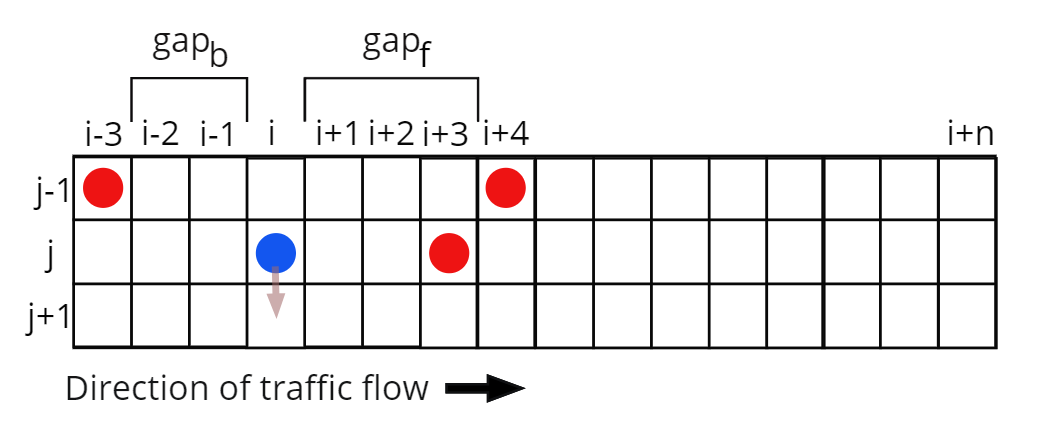
\includegraphics[width= 10cm]{lane1.png}
  \vspace{-0.3cm}
  \caption{Lane Change Dynamics}
    \vspace{-0.2cm}
  \label{fig:lane}
\end{figure}
\end{comment}

From Theorem \ref{th1}, it can be seen that an AV following another AV can attain the highest possible speed, $v_{aa}$, whereas the maximum speed for a HV is the lowest, $v_{h}$ and is independent of the class of the vehicle it trails. Throughout the rest of the paper when we refer to $v_{max}$ we imply the meaning of $v_{max}$ as described in Eqn. \ref{eq:v}. Our model follows the general rules outlined in Fig \ref{fig:ca}, with the some changes to certain rules marked by "\textbf{\textasteriskcentered}
" in Fig.\ref{fig:ca}. These new rules are explained below: 
\begin{figure}[H]
\centering
  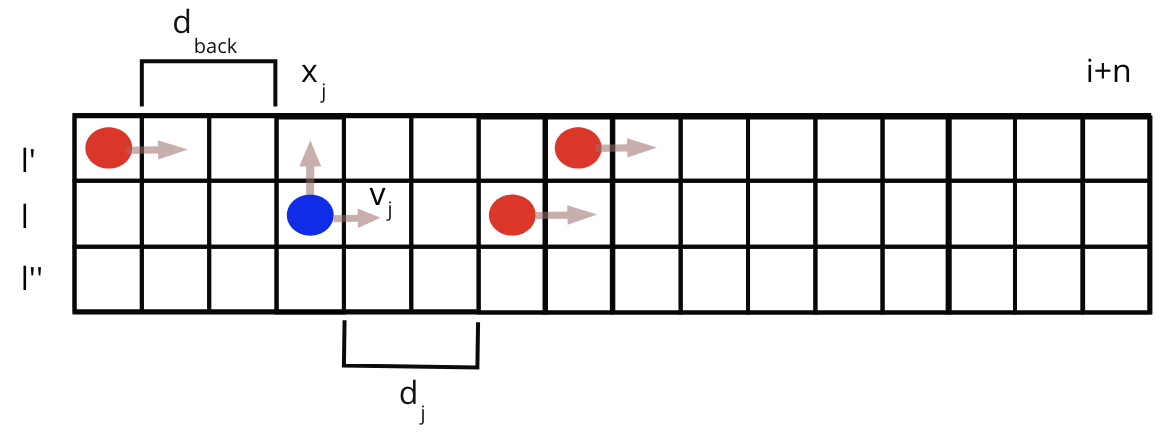
\includegraphics[width= 0.5\textwidth]{l2.png}
  \vspace{-0.3cm}
  \caption{Road - Car grid in Cellular Automata}
    \vspace{-0.2cm}
  \label{fig:lane}
\end{figure}
\begin{itemize}
%\begin{flushleft}
\item \textbf{Rule A:} 
In our model $v_{l'}$  is defined as: $ v_{l'} = min(v_{max}, d_{back})$. Here, $v_{l'}$ represents the potential speed the vehicle can attain if it switches lane from lane $l$ to lane $l'$. If $d_{j}$ is the number of empty cells in front of car in lane $l$. The incentive criterion dictates that the vehicle will switch lanes only and only if:
\begin{equation}
    v_{l'} > d_{j}
\end{equation}
\item \textbf{Rule B: \begin{equation}
        \label{eq:3}
    d_{back} > v_{prev}
\end{equation}}
Once an incentive to switch lanes have been established, the safety criterion implies that the vehicle looks for the car that would be behind it in the target lane, $l'$ Then, it is required that the distance to the previous car, $d_{back}$, is greater than the speed of the previous car, $v_{prev}$ in the target  lane to avoid any collision while switching lanes.
\begin{comment}
\item \textbf{Rule C:}\begin{equation}
        \centering 
         l \rightarrow l' 
    \end{equation}    
After the conditions for both Rules A an B are satisfied, the vehicle has a probability, $p_l$, of switching lanes. This probability is associated with the driver's reluctance to switch lanes even though it would deem plausible; thereby making the model stochastic and realistic. 
The vehicle changes lane once all these conditions are met. It is to be noted that due to the mutually exclusive nature of lane change, vehicles on the middle lane can either move to the left or right lane. For situations like this, preference is given to the left lane in our model.
\end{comment}
%\newpage
%\subsubsection{\textbf{Rules for Forward Propagation}}
\item \textbf{Rule 1 and 2:} {If $v_j < v_{max}$ and the distance to the next vehicle, $d_j$, is greater than $v_j + 1$, the vehicle accelerates and the new speed, $v_j$, is:
\begin{equation}
            v_j = min(min(v_j + 1, v_{max}), d_j) 
\end{equation}
Rule 1 ensures that the vehicle accelerates linearly till it reaches its maximum speed, $v_{max}$, while Rule 2 also makes sure that there is no collision.\\ }
\begin{comment}
\item \textbf{Rule 3:}\begin{equation}
            v_j = v_j - 1 
            \label{eq:3}
    \end{equation}
The vehicle may slow down randomly with a vehicle type dependent braking probability, $p_b$, and the new speed, $v_{j}$ would be given by Eqn. \ref{eq:3}. This rule is included to model erratic driver behaviour in HVs and the lack thereof in AVs; it makes the simulation reflect realistic traffic flow by taking away total determinism from the model.
\item \textbf{Rule 4:} The vehicle moves $v_j$ cells from its initial position in the upstream direction. 
\begin{equation}
            x_j = x_j + v_j
            \label{eq:3}
    \end{equation}
\end{comment}
%\end{flushleft}
\end{itemize}

To summarize, when an AV exhibits \textit{neighbor aware} behaviour, it is aware of the type of vehicle in front of it and changes its velocity as a response limiting its maximum speed, $v_{max}$, while HV behaves indifferently. A consequence of this model is the next corollary.
 \begin{corollary} The velocity of a car, $v_j$ is a function of the type of vehicle under consideration, $t_1$ and the type of vehicle it precedes, $t_2$.
  \[ v_j = f(t_1, t_2) \]
\end{corollary}

It should be also be noted that both behaviors- \textit{opportunistic \text{and} "neighbor aware"}- satisfy the safety constraints and correspond to pure opportunistic and pure random nature. Moreover, since, real-world AV behaviors are not well known as of yet due to the lack of large scale deployment of such vehicles, we cannot be sure of the accuracy of our models.
%Comment: Previous texts commented out ============================= end of comment
\begin{comment}
\begin{itemize}
    \item \textbf{Lane Change Behaviour:} Since AVs are intelligent systems, they are modelled to be completely opportunistic and would always make decisions that optimize their traffic flow parameters. Thus, they will always change lanes given that it is both safe and rewarding to change lanes. HVs, like in previous CA models, behave more `humanly'' in this aspect, because it depends on the \textit{aggressiveness} of the human driver. 
    \item \textbf{Erratic Driving Behaviour:} HVs in our model are prone to velocity fluctuations due to human behavior or due to varying external conditions. This type of \textit{erratic} behaviour does not apply to AVs, since they are well aware of their surroundings and make their decisions of accelerating/deceleration solely based on safety and opportunity. 
    \item \textbf{Maximum Speed:} We have assumed that AVs can attain higher maximum speeds than HVs. The reason behind our assumptions lies in the fact that such vehicles are technologically superior than the HVs. 
\end{itemize}
\end{comment}
\begin{comment}

In our model, we treat the road and the vehicles as two different computational objects. The road is defined as a two-dimensional array, where each array element is a one-dimensional array representing a lane . This data structure is used to create the grid of cells, where our vehicle objects are stored. \cite{CA2}

\begin{figure}[! htb]
 \[
   \begin{gmatrix}[b]
    \mathllap{Lane_1\quad}\hspace{0.2mm}[\hspace{1mm} cell_{11}&cell_{12}&\cdots &cell_{1n}\hspace{1mm}] \hspace{1mm} \\
     \hspace{-2mm}\mathllap{Lane_2\quad}\hspace{1mm}[cell_{21}&cell_{22}&\cdots &cell_{2n}\hspace{1mm}] \hspace{1mm}\\
     & \hspace{10mm} \vdots &  & \\
     \mathllap{Lane_m\quad}\hspace{1mm}[cell_{m1}&cell_{m2}&\cdots &cell_{mn}\hspace{1mm}]\hspace{1mm}\colops
\def\colmultlabel#1{\makebox[1.2em]{$#1$}}
     \end{gmatrix}
    \]
\caption{The Road Data Structure}\label{fig:vulnmatrix}
\end{figure}

Each cell can take one of two values: \textit{None} or \textit{<car object>}; the \textit{None} value represents an empty space on the road and the \textit{<car object>} represents a vehicle. Each vehicle object has the following attributes: 
\begin{enumerate}
    \item Position: defined in the form of cell$_{ij}$, where $i$ is the horizontal distance on the road and $j$ is corresponding the lane number. [$(i,j) \in \mathbb{Z}$]
    \item Vehicle type: either an AV or HV
    \item Longitudinal velocity: an integer value, $v_0$, that represents the number of cells the car travels per update. 
\end{enumerate}

\begin{figure}[H]
\centering
  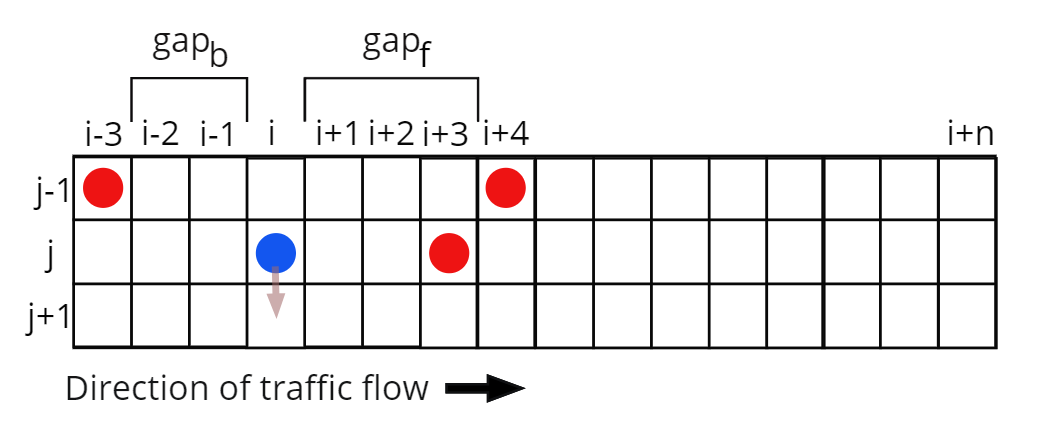
\includegraphics[width= 10cm]{lane1.png}
  \vspace{-0.3cm}
  \caption{Lane Change Dynamics}
    \vspace{-0.2cm}
  \label{fig:lane}
\end{figure}

\textcolor{red}{The rules need to be summarized more and/or add a flow chart summarizing the process\\}

\subsection{Rule for Changing Lanes}
        \begin{enumerate}[(i)]
        \item \textbf{determining target lanes:} the vehicle at position $cell_{ij}$ looks at lanes $j \pm 1$ to verify whether those lanes exist. If the lanes are in bound, the vehicle checks to see whether the position $cell_{ij+1}$ or $cell_{ij-1}$ are empty. It is only when these positions are empty, that  those lanes are considered to be \textit{target lanes} for possible lane change [$lane_{j\pm1} \in Road$ and $cell_{ij\pm1} = \textit{None}$].
        \item \textbf{incentive to change lane:} Once a target lane or target lanes have been established, the vehicle checks to see whether speed in the destination lane, $v_{dest}$ is greater than that of the source lane, $v_{0}$. $$v_{dest} = min(v_{sl}, gap_{f})$$ Here, $gap_f$ represents the the distance to the next car in the destination lane and the $v_{sl}$ represents speed limit of the road. If $v_{dest} > v_{0} $, then the vehicle has incentive to switch lanes [$v_{dest} > v_{src} $].
        \item \textbf{safety check:}  If there is incentive to change lanes, the vehicle looks for the car that would be behind it in the target lane. Then, it is required that the distance to the previous car, $gap_b$, is greater than the speed of the previous car, $v_{prev}$ in the target lane to avoid any collision while switching lanes. [$gap_b > v_{prev}$]. 
        \item \textbf{reluctance to switch lanes:} After all these conditions are met, the vehicle has a probability, $P_{lane}(vtype_0)$, of not switching lanes. This probability is dependent on the type of vehicle, $vtype_0$, under consideration. $$X \sim Random\{0,1\}$$
        \[
        cell_{ij} =
        \begin{cases}
                                   cell_{ij} & \text{if $X < P_{lane}(vtype_0)$} \\
         cell_{ij\pm1}   \hspace{1mm}  & \text{if $X \geq P_{lane}(vtype_0)$}
        \end{cases}
        \]       
        \item \textbf{motion:} If all the conditions of all lane change are met, the vehicle changes position from $cell_{ij}$ to $cell_{j+1}$ or $cell_{ij-1}$. \\

 
 Our lane changing model has the following characteristics- symmetric, stochastic and backward causality- as defined by Rickert et all (1995) \cite{NaSch}. Each vehicle looks at other lanes at all times (rule $(i)$) to check whether it would benefit them to switch lanes (rule $(ii)$). They also make sure it is safe for them to switch lanes by looking back at the car in the destination lane and gauging their speed and distance (rule $(iii)$) [\textit{Backward Causality}]. There is a probability associated with the driver's reluctance to switch lanes even though it would deem plausible (rule $(iv)$) [\textit{Stochastic}]; this probability models realistic traffic as human drivers don't always change lane, and AVs, as intelligent systems, would be opportunistic. Cars remain on their given lane as long as they don't "see" another vehicle in front of them, making the model \textit{Symmetric}. However, due to the mutually exclusive nature of lane change, vehicles on the middle lane can either move to the left or right lane. For situations like this, preference is given to the left lane.
    \end{enumerate}
    
\textcolor{red}{The rules need to be summarized more and/or add a flow chart summarizing the process\\}
    
\subsection{Rule for Forward propagation}
    \begin{enumerate}[(i)]
        \item \textbf{acceleration:} if $v_0 < v(vtype_0)_{max}$ and the distance to the next vehicle, $gap_{n}$, is greater than $v_0 + 1$, the vehicle accelerates and the new speed, $v_f$, is $v_0 + 1$ $[v_f = v_0 + 1]$.
        $$ v_f = min(v_0 + 1, gap_n) $$
        \item \textbf{safety braking:} if the next vehicle is at position $cell_{kj}$, where $k = i + m$, where $m \leq v_0$ , the vehicle brakes to avoid collision and the new speed, $v_f$, is $m - 1$ $[v_f = m - 1]$.
        \item \textbf{stochastic slowing down:} the vehicle may slow down randomly with a vehicle type dependent probability of $P_{brake}(vtype_0)$ and the new speed, $v_f$, is $v_0 - 1$ $[v_f = v_0 - 1]$.
        $$Y \sim Random\{0,1\}$$
        \[ v_{f} =
        \begin{cases}
        v_0   \hspace{1mm}  & \text{if $Y > P_{brake}(vtype_0)$}\\
        v_{0} - 1& \text{if $Y \leq P_{brake}(vtype_0)$} 
        \end{cases}
        \]       
        \item \textbf{gap preference:} the vehicle may have different headway depending on the type of vehicle in front of it, the vehicle may respond to this by either increasing or decreasing its speed. This would put a cap on the maximum speed of the vehicle, $v(vtype_0)_{max} = v_{hway}$. Here, $v_{hway}$ is a function of the type of vehicle under consideration and the type of vehicle of vehicle in front of it, $vtype_{n}$ 
        \begin{equation}
          v(vtype_0)_{max} =  v_{hway}(vtype_{0}, vtype_{n})
          \label{m2v}
        \end{equation}
        We discuss more on the application of this gap preferential velocity in modelling AV behavior on overall traffic flow in later sections.
        \item \textbf{motion:} the vehicle moves $v_f$ cells int the $i$ direction. \\
      
    \end{enumerate}

\hspace{-1.3cm}Rule $(i)$ ensures that the vehicle accelerates linearly till it reaches its maximum speed, $v(vtype_0)_{max}$. The maximum speed for the vehicle is dependent on the type of vehicle - AV or HV- as an effort to model heterogeneous traffic flow. The stochastic slowing down: rule ($iii)$ is included to model erratic driver behaviour in HVs and the lack thereof in AVs; this rule makes makes the simulation reflect realistic traffic flow by taking away total determinism from the model. The rules for forward propagation can be summarized by the following equation:
%\end{comment}



\subsection{\textbf{Gap Preference and Gap Seeking}}

\textcolor{red}{Better explanation and a flow chart\\}

In our model, we have two different types of vehicles comprising the mixed traffic flow -AVs and HVs. We define their different behaviors in the following regards:

\begin{itemize}
    \item \textbf{Lane Change Behaviour:} Since AVs are intelligent systems, they are modelled to be completely opportunistic and would always make decisions that optimize their traffic flow parameters. Thus, they will always change lanes given that it is both safe and rewarding to change lanes. HVs, like in previous CA models, behave more ``humanly'' in this aspect, because it depends on the \textit{aggressiveness} of the human driver. 
    \item \textbf{Erratic Driving Behaviour:} HVs in our model are prone to velocity fluctuations due to human behavior or due to varying external conditions. This type of \textit{erratic} behaviour does not apply to AVs, since they are well aware of their surroundings and make their decisions of accelerating/deceleration solely based on safety and opportunity. 
    \item \textbf{Maximum Speed:} We have assumed that AVs can attain higher maximum speeds than HVs. The reason behind our assumptions lies in the fact that such vehicles are technologically superior than the HVs. 
\end{itemize}


In the experiment, we further consider two types of AV behaviors: \textit{vehicle type indifferent} and \textit{vehicle type aware} - later we will discuss the formation of clusters of the latter scenario. In the \textit{vehicle type indifferent} case, both the HV and AV are not aware of the type of vehicle in front of it. And rule (2iv) from Section 2.3 is not applied. On the other hand, when the AV exhibits \textit{vehicle type aware} behaviour, it is aware of the type of vehicle in front of it and changes its velocity as a response limiting its maximum speed, $v_{max}$, while HV behaves indifferently. We know from Eqn. 4, this new $v_{max}$ is a function of the type of vehicle in consideration, $vtype_0$, and the type of vehicle in front of it, $vtype_n$. Table 2 shows all the possible combinations of this \textit{gap preferential velocity}.

It should be noted that both behaviors satisfy the safety constraints and correspond to pure opportunistic and pure random nature. Moreover, since, real-world AV behaviors are not well known as of yet due to the lack of large scale deployment of such vehicles, we cannot be sure of the accuracy of our models.
\end{comment}
%Comment: Previous texts commented out ============================= end of comment

\subsection{Model Implementation} \\
Both our simulation and analysis program were written in Python3. The graphics for the simulation were made using the Pygame 1.9.6 module. To create our model, we used principles of Object Oriented Programming with the main objects being two Abstract Data Structures: the Road and Car. The implementation of the NaSch CA algorithms was done through passing functions to these data structures and manipulating the control flow of the program. 

%For the analysis part, we recorded all our parameters as text files, which were later processed to plot the graphs. The processing step made extensive use of the matplotlib, numpy, astropy. scipy, csv and random libraries. To make curve fitting models of the Fundamental Diagram, we primarily used the curve\_fit and differential\_evolution functions from scipy.optimize. 

\section{Experiments and analysis}{\label{sec:exp}}

In this section, we discuss about the two simulation experiments that we conducted and the results we obtained from these experiments. The purpose of these experiments was to study the impact of the two models of AV - \textit{"neighbor aware"} and \textit{"opportunistic"} - on the overall traffic flow and better understand any emergent patterns of collective behavior. \textcolor{red}{Mention our results here briefly?}.

In both the experiments, we consider a circular road with three lanes (periodic boundary conditions), each lane comprising of 100 cells. The vehicle objects follow the set of update rules we defined in Section \ref{S:2}. For each simulation, the road starts from empty state. $N$ Vehicles are then distributed randomly on the road with zero initial velocity; the vehicle type is determined stochastically upon allocation, following a binomial distribution with $P(AV)=0.3$, where $P(AV)$ is the probability of a vehicle being an AV (i.e. percentage of AVs).

\subsubsection{\textbf{Experiment 1:}}
\textcolor{red}{Answer to find: is clustering a normal phenomenon? can we design AV behavior that can form self organized clustering?\\}
For experiment 1, we consider three different models of AV: \textit{"neighbor aware", opportunistic} and \textit{base scenario}. Here, the \textit{"neighbor aware"} model of AV behaves according to rules described in Section \ref{ss:1}; the \textit{opportunistic} model of AV behaves similar to HV's but are modeled to be \textit{purely} opportunistic by being incentivized to seek gaps. The \textit{base scenario} model of AV is where an AV behaves \textit{exactly} like a HV, with their behavior being indistinguishable from one another. Table \ref{tbl:x} summarizes the differences between the three models.

\begin{table}[H]
\centering
\begin{tabular}{ |c|c|c|c| } 
 \hline
 Parameter & Neighbor Aware & Opportunistic & Base Scenario  \\ 
  \hline
 $p_{l}(HV)$ & 0.6 & 0.6 & 0.6 \\ 
 $p_{l}(AV)$ & 1 & 1 & 0.6  \\ 
  \hline
 $p_{s}(HV)$ & 0.4 & 0.4 & 0.4  \\ 
 $p_{s}(AV)$ & 0  & 0 & 0.4\\ 
 \hline
 $v_{aa}$ & 5 & 5 & 5  \\ 
 $v_{ah}$ & 4  & 5 & 5\\ 
 $v_h$ & 3  & 4 & 5\\ 
 \hline
\end{tabular}
\caption{Table of parameter values used in the three test cases of Experiment 1 and 2}
\label{tbl:x}
\end{table}

We simulate the traffic flow for each of these models of AV for the same number of simulation time steps for three different densities: $0.08, 0.2 \text{ and } 0.6$- these three densities correspond to a low occupancy state, critical state and high occupancy state for the road respectively. The proportion of AV, throughout the experiment, was kept constant at $P(AV)=0.3$. We record all the key traffic flow parameters and present our results in the following sections.

\subsubsection{\textbf{Experiment 2:}}
\textcolor{red}{Answer to find: does clustering improve traffic flow parameters? \\}
Similar to experiment 1, we again consider three different models of AV: \textit{"neighbor aware", opportunistic} and \textit{base scenario}, but unlike experiment 1, in experiment 2 we increase our system density linearly for each simulation till it reaches the jam density. The trajectory of the system density evolution in the density phase space is determined by $P(AV)$, where state trajectory is a straight line with slope $\frac{\rho_{AV}}{1-\rho_{AV}}$ (see Figure~\ref{fig:lane}). Throughout the simulation, we track this evolution of system density and system throughput (i.e. flux).

We keep the simulation period at each density constant and discard the data from the first fifth of the period to account for system transition from empty to steady state. 
\begin{figure}[H]
\centering
  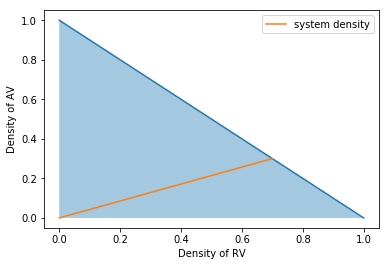
\includegraphics[width= 10cm]{phase1.png}
  \vspace{-0.3cm}
  \caption{Example of system density (\textcolor{orange}{orange}) evolution in allowed phase space (\textcolor{blue}{blue})}
    \vspace{-0.2cm}
  \label{fig:lane}
\end{figure}

\begin{comment}
We consider two lane control scenarios: \textit{AV dedicated lane} and \textit{share lane}. In the first case, we allocate the outer right lane  for AV use only (refer to \ref{fig:vizroad}). In the second case, all lanes are shared by AVs and HVs, and vehicles have no preference over a particular lane. In addition, we consider two different AV behaviors in our experiment: \textit{vehicle type aware} and \textit{vehicle type indifferent}. The experiment will examine behaviors of mixed traffic flow under the four combinations of control and behavior scenarios. For the rest of the paper, we will refer to the \textit{share lane} case as $R1$, \textit{AV dedicated lane} case as $R2$, the \textit{vehicle type aware} as as $M1$ , and the \textit{vehicle type indifferent} as as $M2$. Our experiment comprises of four scenarios: $R1M1$, $R1M2$, $R2M1$ and $R2M2$.

\begin{figure}[H]
\begin{center}
\begin{tikzpicture}
\coordinate (O) at (0,0);
\draw (O) circle (2.2);
\draw (O) circle (1.6);
\draw (O) circle (1);
\draw (O) circle (0.4);
\draw[decoration={text along path,reverse path,text align={align=center},text={Dedicated Lane}},decorate] (0.6,0) arc (0:240:0.6);
\draw[decoration={text along path,reverse path,text align={align=center},text={Share Use Lane }},decorate] (1.2,0) arc (0:180:1.2);
\draw[decoration={text along path,reverse path,text align={align=center},text={Share Use Lane}},decorate] (1.8,0) arc (0:180:1.8);
\end{tikzpicture}
\end{center}
\caption{The road in the \textit{AV dedicated lane} regime}\label{fig:vizroad}
\end{figure}
\end{comment}
\begin{comment}
% From Eqn. \ref{q}, we can write our system throughput, $q_s$ as:
% \begin{equation}
%     q_s = \rho_s \frac{\sum_{i=1}^{N} v_{0}(i)}{N} 
%     \label{qa}
% \end{equation}
% Using Eqn. \ref{den}, we can rewrite, $q_s$ as:
% \begin{equation}
%     q_s = \frac{1}{L} \sum_{i=1}^{N} v_{0}(i)
%     \label{qb}
% \end{equation}
% Since, $\frac{1}{L}$ is a constant, let us use $L_0 = \frac{1}{L}$ from now on for ease of algebra. We can, therefore, write $q_s$ as:
% \begin{equation}
%     q_s = L_0 (v_{0}(1) + v_{0}(2) + v_{0}(3) + \hdots + v_{0}(N))
%     \label{qc}
% \end{equation}
% Here $v_{0}(i)$ is the velocity of the $ith$ vehicle. Since, we know each vehicle is either an AV or HV, let $v_{o}(AV)(i)$ and $v_{o}(HV)(j)$ represent the speed of $ith$ AV and $jth$ HV respectively. Since, the number of vehicles, $N$, in each time period is constant, the number of AVS, $num(AV)$ and $num(HV)$ can be simplified into Eqn. \ref{binb} and \ref{binc} using Eqn. \ref{bin} \ref{prob} and \ref{bina}:
% \begin{equation}
%     num(AV) = NP(AV) 
%     \label{binb}
% \end{equation}
% \begin{equation}
%         num(HV) = NP(HV)
% \label{binc}
% \end{equation}
% Thus, we can rewrite Eqn. \ref{qc} as:
% \begin{equation}
%     q_s = L_{0} (\sum_{i=1}^{num(AV)} v_{0}(AV)(i) + \sum_{j=1}^{num(HV)} v_{0}(HV)(j))
%     \label{qd}
% \end{equation}
% Eqn. \ref{qd} models the flux of mixed traffic flow in the $M2$ model of AV as the maximum speed of each type of vehicle $v_{max}$ is independent of each other and are constant (condition for $M2$). We use the following values for each vehicle type's $v_{max}$ in our experiment. 
% \begin{equation}
%     v_{max}(AV) = 5
% \end{equation}
% \begin{equation}
%     v_{max}(HV) = 4
% \end{equation}
% Therefore, we can calculate the the maximum throughput, $q_{max}$, for this scenario using the following equation:
% \begin{equation}
%     q_{max} = L_{0} (\sum_{i=1}^{num(AV)} v(AV)_{max}(i) + \sum_{j=1}^{num(HV)} v(HV)_{max}(j))
%     \label{qe}
% \end{equation}
% Eqn. \ref{qe} can be simplified into:
% \begin{equation}
%     q_{max} = L_{0} (num(AV) v(AV)_{max} + num(HV) v(HV)_{max})
%     \label{qd2}
% \end{equation}
% Similarly, we can derive the flux equation for the \textit{vehicle type aware} model of AV ($M1$). Under this model, the $v_{max}$ of AVs are dependent on the type of vehicle they follow [See Eqn. \ref{m2v}].
% \begin{equation}
%         v(AV)_{max}=
%         \left\{ \begin{array}{ll}
%              v_{AV} & \text{if } v_{hway}(AV, AV) \text{ or } v_{hway}(AV, cell) \\
%              v_{HV} & \text{if } v_{hway}(AV, HV) 
%         \label{vman}    
%         \end{array} \right.
% \end{equation}
% We used the following values in our experiment for this model:
% \begin{equation}
%     v_{max}(HV) = 3
% \end{equation}
% \begin{equation}
%     v_{AV} = 5
% \end{equation}
% \begin{equation}
%     v_{HV} = 4
% \end{equation}
% Let $P(AV-AV)$, $P(AV-HV)$ and $P(AV-cell)$ be the probability that a given AV is trailing another AV, HV or no vehicle respectively. Since, the road is circular, we can assert:
% \begin{equation}
%     P(AV-HV) + P(AV-AV) + P(AV-cell) = 1
% \end{equation}
% Since, the number of cars, $N$ are constant. The number of AVs trailing other AVs, $num(AV-AV)$, can be found by the following equation:
% \begin{equation}
%     num(AV-AV) = N P(AV) P(AV-AV) = num(AV) P(AV -AV)
% \end{equation}
% Similarly, the number of AVs trailing HVs, $num(AV-AV)$, and trailing no vehicle, $num(AV-cell)$, can be calculated by:
% \begin{equation}
%     num(AV-HV) = N P(AV) P(AV-HV) = num(AV) P(AV -HV)
% \end{equation}
% \begin{equation}
%     num(AV-cell) = N P(AV) P(AV-cell) = num(AV) P(AV -cell)
% \end{equation}
% Thus, we can write the flux equation for the $M1$ model for AV as:
% \begin{equation}
%     q_s = L_{0} [\hspace{-4mm}\sum_{i=1}^{num(AV-AV)}\hspace{-7mm} v_{0}(AV)(i) + \sum_{i=1}^{num(AV-HV)}\hspace{-7mm} v_{0}(AV)(i) + \sum_{i=1}^{num(AV-cell)} \hspace{-7mm}v_{0}(AV)(i)+ \sum_{j=1}^{num(HV)}\hspace{-7mm} v_{0}(HV)(j)]
%     \label{qf}
% \end{equation}
% Let $num(AV*)$ represents the number of AVs trailing behind another AV or no vehicle. 
% \begin{equation}
%     num(AV*) = (num(AV-AV) + num(AV-cell)
%     \label{cc}
% \end{equation}
% Using, Eqn. \ref{qf}, \ref{vman} and \ref{cc}, we can deduce that the maximum throughput, $q_{max}$, for this scenario would be: 
% \begin{equation}
%     q_{max} = L_{0} [(num(AV*)v_{AV} +  num(AV-HV)v_{HV} + num(HV)v(HV)_{max}]
%     \label{qfmax}
% \end{equation}

% We introduce a parameter, $G$, that counts the total number of cells occupied by and enclosed by a certain vehicle type. For example, in the situation presented in Fig. \ref{fig:gap} , $G(AV)$ would be 7 as there are 2 AVs and 5 empty cells enclosed by them.
% \begin{figure}[H]
% \centering
%   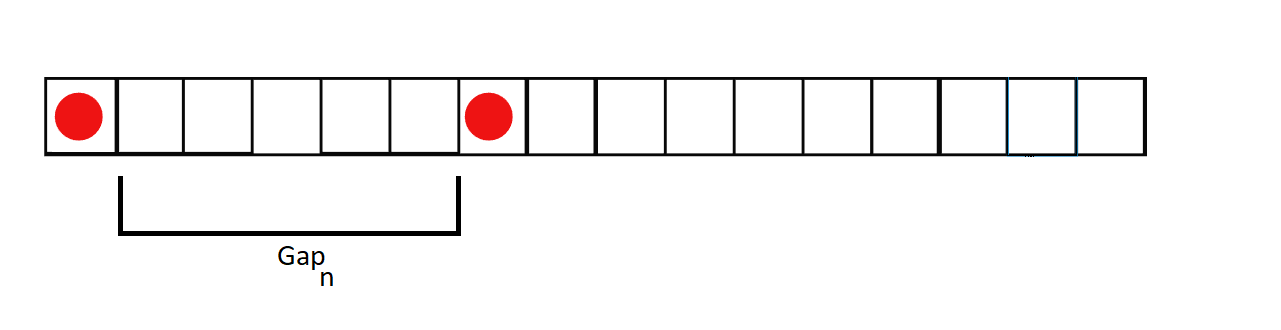
\includegraphics[width= 10cm]{gap.png}
%   \vspace{-0.6cm}
%   \caption{Two AVs seperated by $gap_n$ cells}
%     \vspace{-0.2cm}
%   \label{fig:gap}
% \end{figure}
% In general, if there are $m$ AVs and $gap_n$ empty cells in between them, then $G(AV)$ can be calculated as follows:
% \begin{equation}
%     G(AV) = m + gap_n
%     \label{gapn}
% \end{equation}
% Thus, we can state that:
% \begin{equation}
%     G(AV) + G(HV) = L
% \end{equation}
% This parameter is pivotal to understand which regime would maximize the system throughput for a given system density. The regime's $R1$ and $R2$ are only different in that $R2$ has a dedicated lane and $R1$ does not. This means that the only difference to the system throughput for the regimes under the same AV model and same configuration would be due to the dynamics of the vehicles on the outermost right lane, \textit{test lane}, - \textit{dedicated} for $R2$ and \textit{Share Use} for $R1$.

% Lets assume these two regimes with the same number of total vehicles, $N$ distributed in the same fashion on the other two lanes except for the \textit{test lane}. Let $q_{other}$ be the throughput for the other two lanes and $q_t$ be the throughput on the \textit{test lane}. Therefore, we can say:
% \begin{equation}
%     q_s = q_{other} + q_t
% \end{equation}
%  Since, we assume same conditions in both $R1$ and $R2$, $q_{other}$ would be the same for both the regimes. Let the number of vehicles on the test lane be $N_0$, where $N_0 < N$. Therefore, we can find the number of AVs on the test lane, $num(AV)_0$ and similarly the number of HVs, $num(HV)_0. 
 
%  Considering AV model $M2$: 
%  For regime, $R1$, we can use Eqn. \ref{qd} the throughput, $q_t(R1)$ is:
% \begin{equation}
%     q_t(R1) = 3 L_{0} [\sum_{i=1}^{num(AV)_0} v_{0}(AV)(i) + \sum_{j=1}^{num(HV)_0} v_{0}(HV)(j)]
%     \label{qdi}
% \end{equation}
% Since under regime, $R2$, the test lane is \textit{dedicated} this implies that there be no HVs in the test lane. Under the current model, the only time Hvs can access this lane is to avoid collisions, which means its only at very high system densities that the test lane in $R2$ accomodates HVs. We do not consider those cases for this part of the analysis. For the most part, we can define $q_t(R2)$ as:
% \begin{equation}
%     q_t(R2) = 3 L_{0} \sum_{i=1}^{num(AV)_0} v_{0}(AV)(i) 
%     \label{qdIi}
% \end{equation}
% Therefore, it can thus now be stated that whenever $q_t(R2) > q_t(R1)$, having a dedicated lane would improve the overall traffic flow. In the case, that there are equal number of cars in the test lane and both regimes are in equilibrium, with the cars in the test lane travelling at their maximum speed. $R2$ would always perform better than $R1$ because $ q_{tmax}(R2) >  q_{tmax}(R1)$ for all values of P(AV).
% \begin{equation}
%     q_{tmax}(R2) = 3 L_{0} N_0 P(AV)  v(AV)_{max}
%     \label{qdIid}
% \end{equation}
% \begin{equation}
%     q_{tmax}(R1) = 3 L_{0} N_0 [ P(AV)  v(AV)_{max} +  P(HV)  v(HV)_{max}]
%     \label{qdIid}
% \end{equation}
% In more realistic situations, this conclusion does not hold. The better performing regime is rather decided by the number of cars in the test lane.
% Our system started off with $N_0$ vehicles on the test lane, which was the same for both the regimes. Over some time these numbers would differ, let $N_{R1}(t)$ represent the number of vehicles in the test lane in $R1$ as a function of time and similarly $N_{R2}(t)$ represents that of $R2$. 
% \begin{equation}
%     N_{R1}(0) = N_{R2}(0) = N_0 = N_{R1}(AV)(0) + N_{R1}(HV)(0) = N_{R2}(AV)(0) + N_{R2}(HV)(0)
%     \label{init}
% \end{equation}
% In both these regimes, there would be both cars switching into this lane and out of this. In $R2$, it is required that all the HVs leave the lane as soon as possible and no HV enter the lane.
% \begin{equation}
% \frac{dN_{R2}(AV)(t)}{dt} = m < 0
% \end{equation}
% On the other hand there is no such constraint for $R1$.
% \begin{equation}
%  \frac{dN_{R1}(AV)(t)}{dt} = k 
% \end{equation}
% Now, if we consider the rate of lane change of AV from test lane. 
% \begin{equation}
%      \frac{dN(AV)(t)}{dt}  =  \frac{dN(AV_{up})(t)}{dt} +  \frac{dN(AV_{dn})(t)}{dt} 
% \end{equation}
% Here, $ \frac{dN(AV_{up})(t)}{dt}$ represents and the rate at which number of cars leaving the test line in time $t$ and $frac{dN(AV_{dn})(t)}{dt}$ represents the opposite.
% In both $R1$ and $R2$, it can be argued that the resultant rate for AV is the same.
% \begin{equation}
%      \frac{dN_{R1}(AV)(t)}{dt}  =  \frac{dN_{R1}(AV)(t)}{dt} = C
% \end{equation}
% Therefore, it is this lane change rate to and from the test lane that determines which regime is more effective for a given $P(AV)$ and system density and the regime that has the lower resultant rate of vehicles coming into the test lane would have the best throughput.
\end{comment}

\subsection{\textbf{Clustering and Lane Formation}}
\textcolor{blue}{Structure: \\ what is clustering? how did we quantify? \\is clustering a regular phenomenon? if not why is it not? what are the factors behind clustering? \\which AV behavior results in clustering and how significant is it compared to other models? \\How do our results prove our explanation?\\}
The purpose of experiment 1 is to understand self-organization phenomenon of AV into clusters and lanes (which we call lane formation). We define them as follows: 
\begin{deflist}
\hspace{-1cm}\textbf{$\bullet$ Cluster:} Has 4 or more AVs each at most 3 cells apart \\
\end{deflist}
\vspace{-0.5cm}
\begin{deflist}
\hspace{-1cm}\textbf{$\bullet$ Lane Formation:} Has 4 or more AVs trailing each other on the same lane with no HVs in between them
\end{deflist}

In both cases, we observe interesting self-organization phenomena: as time passes by, AVs organize them into clusters and form lanes without any centralized command. Figure~\ref{fig:cls0} and \ref{fig:cls} provide snapshots of this phenomenon for both cases. In the case $R1M1$ (AVs are type-aware), we find the number and size of such clusters and lanes are both larger than the case $R2M2$. This may be verified from the distribution of cluster sizes in Figure~\ref{clm1} and \ref{clm2} .

We hypothesize that the formation of clusters and lane is due to the opportunistic nature of AVs, modeled through both its gap seeking and braking behaviors as we described above. In the type aware model of AVs, it is actually rewarding to the AV to trail behind another AV as they can achieve smaller headways. This leads to the phenomenon of lane formation as AVs are essentially incentivized to change lanes aggressively and overtake HVs to seek and follow a peer. The fact that $R1M1$ case has stronger clustering to certain extent verify this hypothesis, because AVs have better incentives in $R1M1$ due to their awareness of vehicle types.

\begin{figure}[H]
\centering
\hspace{-0.1cm}
  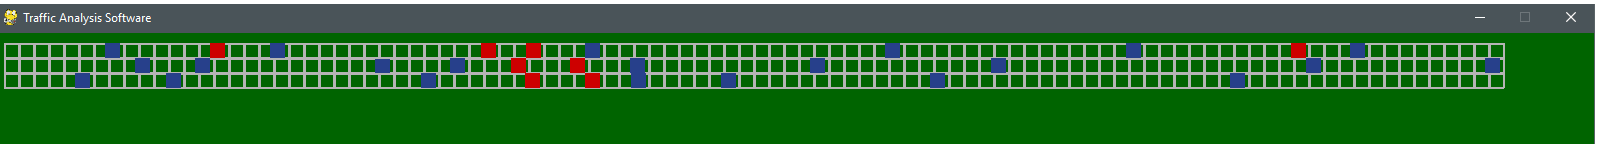
\includegraphics[width= 18cm]{cls.png}
  \vspace{-0.6cm}
  \caption{A cluster of 6 AVs (red)}
    \vspace{-0.2cm}
  \label{fig:cls0}
\end{figure}
\begin{figure}[H]
\centering
\hspace{-0.1cm}
  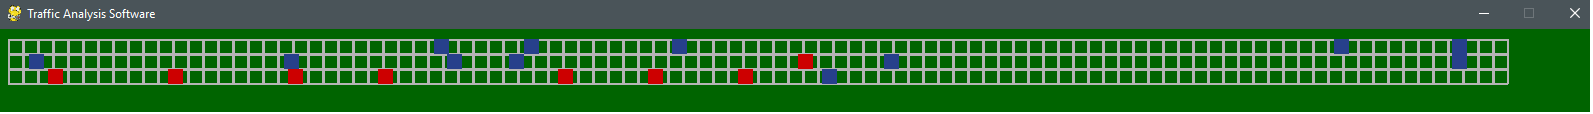
\includegraphics[width= 18cm]{clslane.png}
  \vspace{-0.6cm}
  \caption{A self-organized lane of 7 AVs (red)}
    \vspace{-0.2cm}
  \label{fig:cls}
\end{figure}


%comment start: ==============================================================
\begin{comment}

\begin{figure}[H]
  \centering
  \begin{minipage}[b]{0.4\textwidth}
    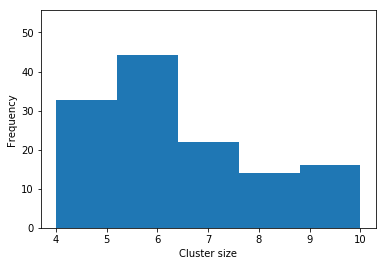
\includegraphics[width=\textwidth]{clsm1.eps}
    \caption{Distribution of cluster sizes in $R1M1$}
    \label{clm1}
  \end{minipage}
  \hfill
  \begin{minipage}[b]{0.4\textwidth}
    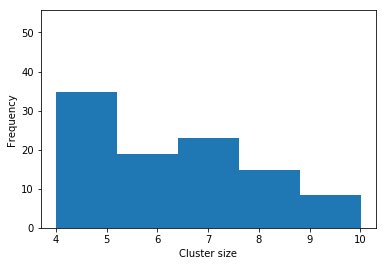
\includegraphics[width=\textwidth]{clsm22.eps}
    \caption{Distribution of cluster sizes in $R1M2$}
    \label{clm2}
  \end{minipage}
\end{figure}

In both cases $R1M1$ and $R1M2$, the maximum speed of AVs are larger than the maximum speed of HVs. We argue that the average speed of vehicles in $R1M1$ would be less than or equal to the average speed of vehicles in $R1M2$. This is because of two reasons:\\
\begin{enumerate}
    \item the maximum speed of HVs in $M2$ is greater than that of $M1$.
    \item  the average maximum speed of AVs in $M1$ is less than or equal to that of $M2$'s.\\
\end{enumerate} 
%\begin{equation}
  %  \overline{v(M1)} \leq \overline{v(M2)}
  %  \label{leq}
%\end{equation}
\\ \\
Since, the system throughput, $q_{s}$ is directly proportional to the speed of the traffic flow. The flux, $q_{s}(M1)$, in $M1$ must be less than or equal to the flux, $q_{s}(M2)$, in $M2$. 
\begin{equation}
    q_s(M1) \leq q_s(M2)
\end{equation}
However, since the maximum speed of HVs in are greater in model $M1$ than $M2$, when the system is at equilibrium, the gap, $gap_n$, between two consecutive HVs would smaller in $M1$ than in $M2$. This is due to the fact that at equilibrium the HVs would be travelling at their highest speeds, and as their maximum speed in $M1$ is less than that in $M2$, the HVs would take up less space while moving in $M1$ when compared with $M2$.
\begin{equation}
    gap_n(M1) < gap_n(M2)
    \label{gap}
\end{equation}
This condition gives AVs greater mobility in $M1$ than in $M2$ as there is more space in on the road for AVs . This property combined with the opportunistic nature of AV and the fact that they can attain smaller headways and thus higher speed by following other AVs ($v(AV-AV)_{hway} > v(AV-AV)_{hway}$) explains why both the numbers and sizes of these self-organized clusters and lanes are greater in $M1$ compared to $M2$.

The total number of such \textit{clusters} and \textit{lanes} reach a maximum over time in our model. This is due to the fact that the total density increases with time as well, and this leads to fewer cells and lanes open to AVs, which means their efforts of clustering and/or forming lanes becomes more and more limited. This rate of convergence to equilibrium is higher in $M2$ for than $M1$ and is due to the same reason why the cluster sizes are smaller in $M2$ - fewer empty cells in between HVs in $M1$ than $M2$ and higher maximum speed of HV in $M1$ compared to $M2$.

When the system is at equilibrium, the marginal benefit of lane change is greater for $R1M1$ than $R1M2$ due to \textit{vehicle type aware} phenomenon.

\begin{figure}[H]
\centering
  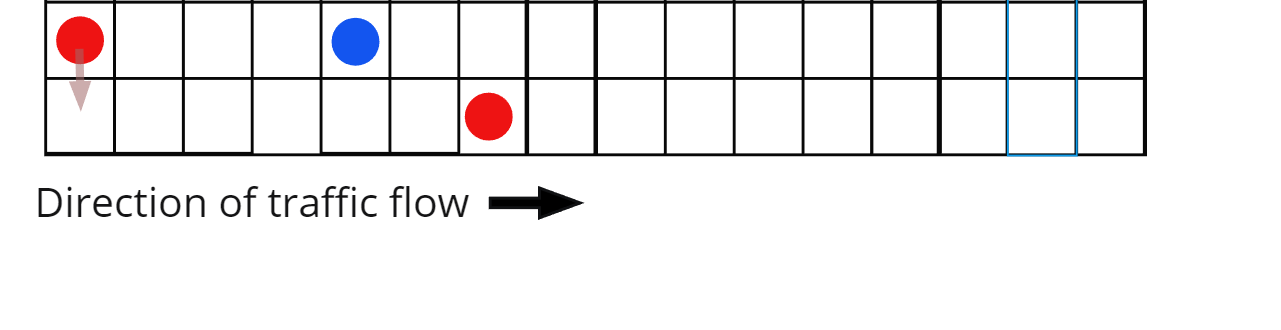
\includegraphics[width= 10cm]{hw.png}
  \vspace{-0.6cm}
  \caption{AV (red) trailing HV (blue) about to change lane}
    \vspace{-0.2cm}
  \label{fig:lanehw}
\end{figure}
In the scenario illustrated by Fig. \ref{fig:lanehw}, if the system is at equilibrium, then the AV trailing the HV has speed, $v(AV)_{max} = v_{hway}(AV, HV)$, upon lane change, the new speed of the AV would be $v(AV)_{max} = v_{hway}(AV, AV)$. Since $ v_{hway}(AV, AV) >  v_{hway}(AV, HV)$, the overall speed as well as throughput of the system would both increase.

We remark that model $R1M1$ may likely be a better approximation to the reality, as sensing and communication capabilities likely make AVs aware of other AVs in its neighborhood. The simulation here indicates the possibility of self-organized clustering and lane forming phenomenon without a centralized control.
\end{comment}
%comment end: ======================================================================

\subsection{Flux of Mixed Flow}

\textcolor{blue}{Structure: \\Introduce this section as results from experiment 2 \\experimental data  \\talk about how we got the plots \\Show FD's for three cases \\show individual FDs for AV and RV \\Analyze the plots \\Answer whether clustering improved traffic flow or not? \\Explain why or why not}
\begin{figure}[H]
\centering
  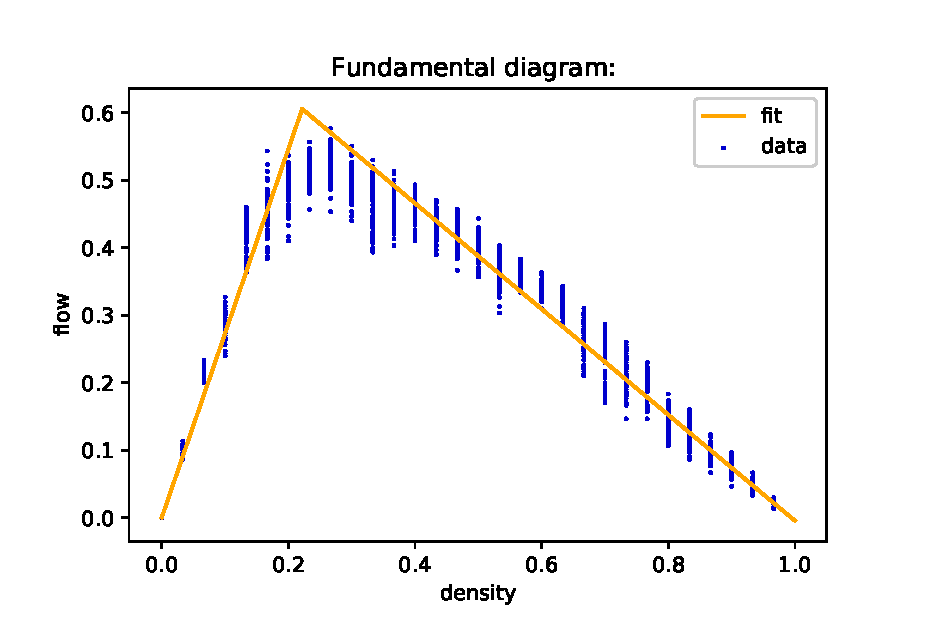
\includegraphics[width= 10cm]{fdfitr2m1.eps}
  \vspace{-0.6cm}
  \caption{Piecewise linear fit of fundamental diagram}
    \vspace{-0.2cm}
  \label{fig:fdtria1}
\end{figure}
We also compare the flux of mixed traffic flow in all scenarios (see Figure~\ref{fig:fdtri} through Figure~\ref{rvfd}). Once the simulation is done, we use a modified Linear Regression method to fit the plot, where the fit is specified to be a piecewise linear function. Figure~\ref{fig:fdtria1} shows an example of the fit.

\begin{table}[H]
\centering
\begin{tabular}{ |p{4cm}||p{3cm}|p{2.5cm}|p{2.5cm}|  }
 \hline
 \multicolumn{4}{|c|}{Experiment Data} \\
 \hline
  &Neighbor Aware  &Opportunistic &Base Scenario \\
 \hline
 Critical Density &   0.20  & 0.16   &0.22 \\
 Maximum Flow &0.53 & 0.57&  0.61 \\
  \hline
 Free flow Speed   & 2.66    &  3.56 &   2.73 \\
 Wave Speed    &-0.66 & -0.68 &  -0.78 \\
  \hline
 Critical Density, RV &   0.15  & 0.11   &0.12 \\
 Maximum Flow, RV &0.37 & 0.39&  0.29\\
  \hline
 Critical Density, AV &   0.09  & 0.10   &0.10 \\
 Maximum Flow, AV &0.28 & 0.22&  0.39 \\
 \hline
\end{tabular}
\caption{Key traffic characteristics in each scenario}
\label{table:sas}
\end{table}


Our results show that $R2M2$ has the best overall throughput, and $R2$ overall perform better than $R1$ in our simulation setting. This is not surprising, considering that dedicated lane would suppress the conflicts between AVs and HVs, and allow AVs to move more efficiently. In this case, the opportunistic behavior of AVs seem to play a negative role in system throughput, due to the extra lane changes induced. As expected $M2$ model of AV improved overall traffic flow as compared to $M1$. Figure~\ref{fig:fdtri} shows the fundamental diagrams for all the scenarios.

\begin{figure}[H]
\centering
  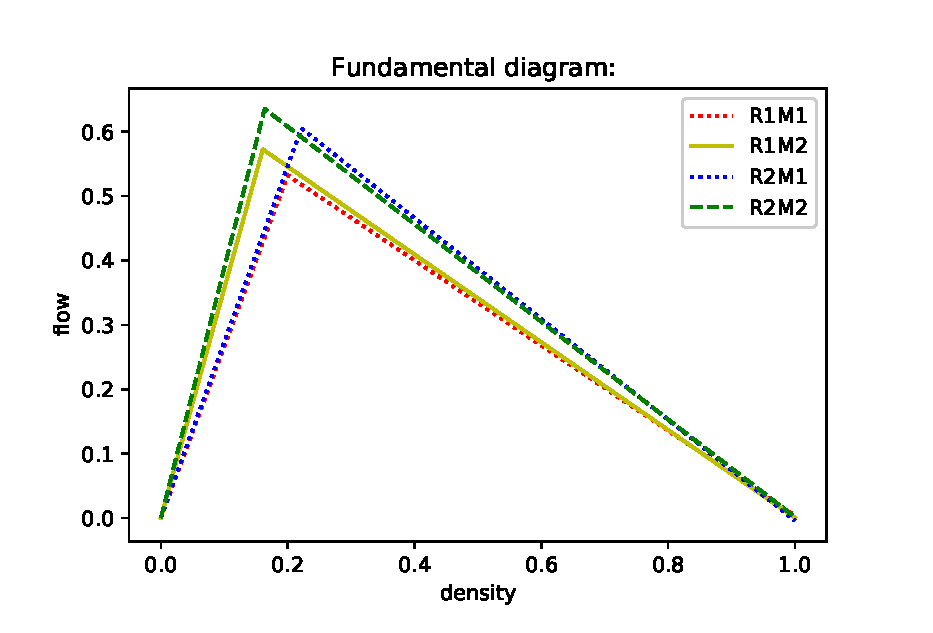
\includegraphics[width= 10cm]{tricomp}
  \vspace{-0.6cm}
  \caption{Fundamental Diagram}
    \vspace{-0.2cm}
  \label{fig:fdtri}
\end{figure}

Fig. \ref{AVFD} and \ref{rvfd} show the fundamental diagrams for the AV class only and HV class only for each of the experimental cases. The AVs performed better under $R2$ while the RVs did better under $R1$ as expected.
\begin{figure}[H]
  \centering
  \begin{minipage}[b]{0.4\textwidth}
    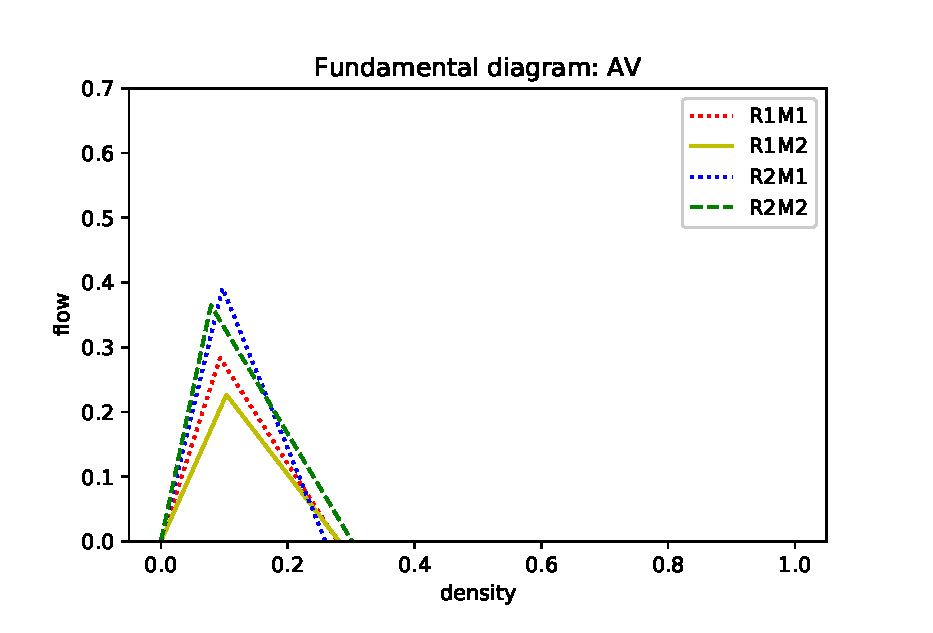
\includegraphics[width=9cm]{tricompav.eps}
        \vspace{-1cm}
    \caption{\hspace{-0.3cm}Fundamental Diagram of AV}
    \label{AVFD}
  \end{minipage}
  \hfill
  \begin{minipage}[b]{0.4\textwidth}
    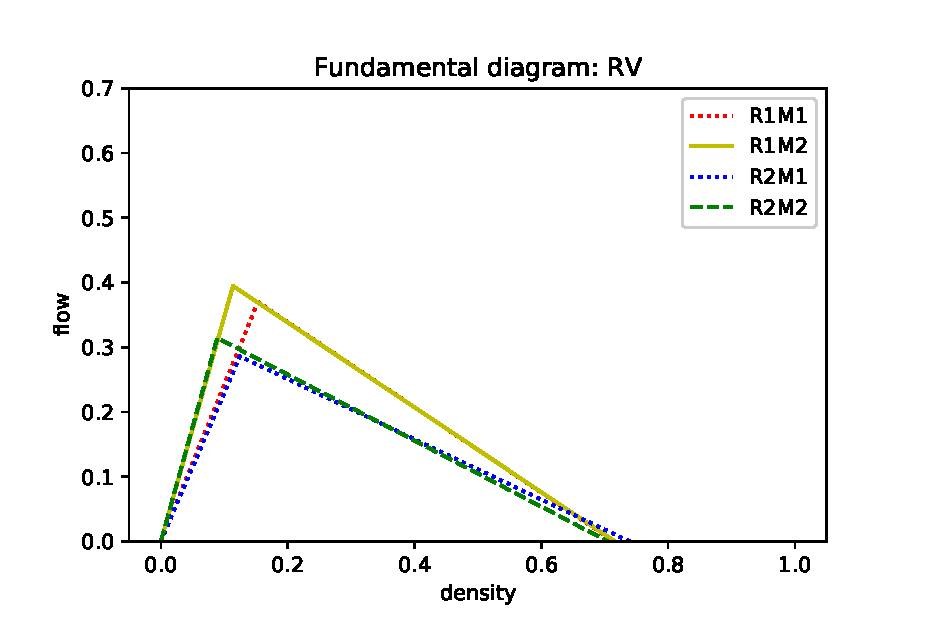
\includegraphics[width=9cm]{tricomprv.eps}
        \vspace{-1cm}
    \caption{\hspace{-0.3cm}Fundamental Diagram of RV}
    \label{rvfd}
  \end{minipage}
\end{figure}

Since overall traffic flow was better under the $R2$, this suggests that the rate at which vehicles entered the test lane in $R2$ (i.e. the dedicated lane) must have been lower than that of $R1$. This is confirmed to be to true as shown by Figure~\ref{fig:lamndtri}. $R2M2$ has the lowest flow rate while $R1M1$ has the highest rate. From Figure~\ref{fig:fdtri}, we can see that $R2M2$ has the best flow characteristics and $R1M1$ has the worst as expected.

\begin{figure}[H]
\centering
  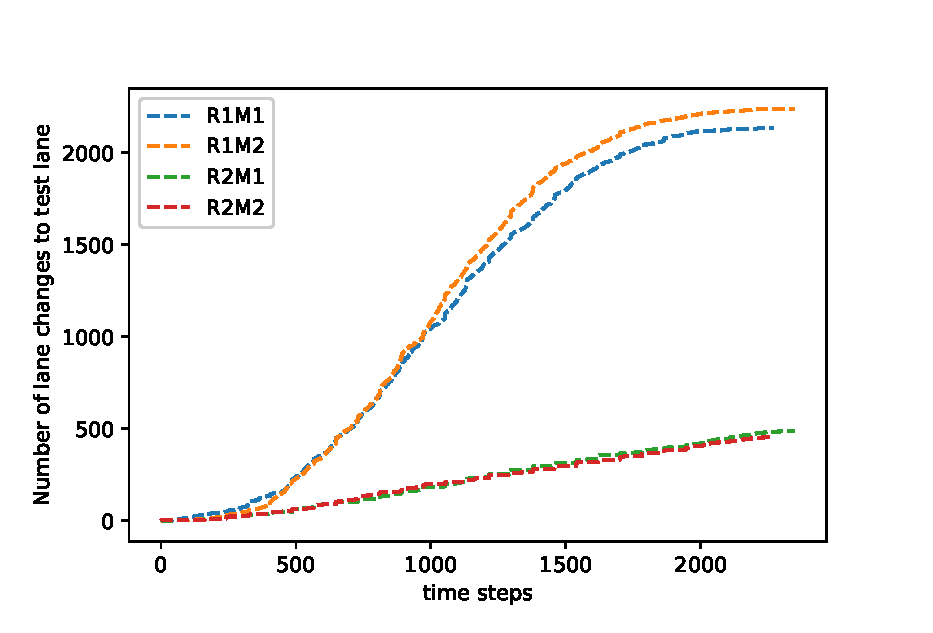
\includegraphics[width= 10cm]{lanecomprv.eps}
  \vspace{-0.6cm}
  \caption{Number of lane changes to test lane over time}
    \vspace{-0.2cm}
  \label{fig:lamndtri}
\end{figure}


Table \ref{table:sas} summarizes the key traffic flow parameters obtained from our experiments. The values indicate that the free flow speed for both $M1$ and $M2$ remained roughly constant across all scenarios. However, the maximum flow under $R2$ was greater than that under $R1$. On the other hand, the wave speed under both $R1$ and $R2$ remained approximately the same independent of the model of AV.


\section{\textbf{Conclusion}}
\textcolor{red}{Needs some change \\}
In this paper, we investigate behaviors of mixed traffic flow of AVs and HVs through simulation experiments. The major purpose is to understand the relation between opportunistic behaviors of AV and formation of clusters and lanes without centralized control. For this purpose, we propose a new cellular automata model to account for potential behaviors difference between AVs and HVs. Notably, the opportunistic character of AVs are modeled through their gap seeking behaviors and awareness of neighboring vehicle types. Simulation experiments were conducted in four scenarios, which compare the clustering process and traffic flow performance with and without opportunistic AVs, and with and without dedicated AV lane.

One major finding of this research, which is intriguing, is the self-organized formation of AV clusters and lanes without any centralized control. Such phenomena are observed in our simulation experiments even no dedicated AV lane is in place. This may suggest clustering as an intrinsic property of mixed HV and AV flow. We postulate such self-organized phenomena is due to the incentives that AVs perceive to seek and partner with peer AVs. When AVs are opportunistic, such effect is reinforced, as seen in our experiment. If the postulation is confirmed to be true through further simulation or field experiments, it may suggest the possibility of regulating mixed HV-AV flow through designing or inducing decentralized incentives, instead of performing centralized coordination. Our research also compares the mixed flux in all scenarios, and the positive effect of dedicated lane is confirmed. 

The findings of this paper may serve as initial evidence to the self-organization in mixed flow of AVs and HVs. We recognized the proposed model is by no means realistic in the quantitative sense. In addition, as AVs haven't been launched in large scale in the real world and existing data is limited, their opportunistic behavior just represent on possibility we deem likely. In future works, as more data become available, it is desirable to model the decision-making of AVs more realistically, and further verify the finding in this paper.

\section{Acknowledgement}

This research is partly supported by a Seed Grant from Hurricane Resilience Institute (HuRRI). 

%\section{References}



%\bibliographystyle{model1-num-names}
%\bibliography{sample.bib}

%% Authors are advised to submit their bibtex database files. They are
%% requested to list a bibtex style file in the manuscript if they do
%% not want to use model1-num-names.bst.

%% References without bibTeX database:

%\begin{thebibliography}{00}

%\bibitem{CAb} Wolfram,  S.,  Theory  and  Applications  of  Cellular  Automata,  World  Scientific,  NewYork, NY, 1986. 
%% \bibitem must have the following form:
 %\bibitem{CA} Nagel, K. and M. Schreckenberg, (1992) "A cellular Automaton Model for Freeway Traffic," Journal de Physique, Vol 2, pp.2221-2229.
 
 %\bibitem{CA2} Nagel, K.( 1996), "Particle Hopping Models and Traffic Flow Theory," Physical Review E," Vol. 3, No. 6, pp. 4655-4672
 
 %\bibitem{NaSch} Rickert, M., Nagel, K., Schreckenberg, M. and A. Latour, (1995), "Two Lane Traffic Simulations using Cellular Automata", Physica A, submitted
 
%\bibitem{3lane} K.  Daoudia,  N.  Moussa,  Numerical  simulations  of  a  three-lane  trafficmodel  using  cellular  automata,  Chinese  journal  of  physic,  Vol.  41,  No.6, December 2008, pp. 123-127

 %\bibitem{agg} X. G. Li, B. Jia, Z. Y. Gao, and R. Jiang, “A realistic two-lane cellular
%automata traffic model considering aggressive lane- changing behavior
%of fast vehicle,” PhysicaA, vol. 367, pp. 479– 486, 2006
 
%\end{thebibliography}

\newpage

\bibliographystyle{plain}

\bibliography{ref}


\end{document}
